\subsection{Lipschitz constants of common loss functions}\label{sec:lossboundsproofs}

    \begin{table}%[]
        \hspace{-0.7cm}
        \begin{tabular}{|c|ccc|}
        \hline
            Loss & Hyper-parameters &  $\Loss(\yhat,y)$ & Lipschitz bound $L$\\
            \hline
            \hline
            \makecell{Softmax Cross-entropy} & temperature $\tau>0$ & $y^T\log{\text{softmax}(\yhat/\tau)}$ & $\sqrt{2}/\tau$\\
            \hline
            \makecell{Cosine Similarity} & bound $X_\text{min}>0$ & $\frac{y^T\yhat}{\max(\|\yhat\|, X_\text{min}}$ & $1/X_\text{min}$\\
            \hline
            \makecell{Multiclass Hinge} & margin $m>0$ & $\{\text{max}(0,\frac{m}{2} - \yhat_i . y_i)\}_{1\leq i \leq K}$ & 1\\
            \hline
            \makecell{Kantorovich-Rubenstein} & N/A & $\{\yhat,y\}$ & 1\\
            \hline
            \makecell{Hinge Kantorovich-Rubenstein} & \makecell{margin $m>0$\\ regularization $\alpha > 0$} & $\alpha . \Loss_{MH}(\yhat,y) + \Loss_{MKR}(\yhat,y)$ & $1+\alpha$\\
            \hline
        \end{tabular}
        \caption{Lipschitz constant of common supervised classification losses used for the training of Lipschitz neural networks with $k$ classes. Proofs in Section~\ref{sec:lossboundsproofs}.}
        \label{tab:cst_lip_loss}
    \end{table}
    
This section contains the proofs related to the content of Table~\ref{tab:cst_lip_loss}. Our framework wraps over some losses found in deel-lip library, that are wrapped by our framework to provide Lipschitz constant automatically during backpropagation for bounds.

\paragraph{Multiclass Hinge} This loss, with min margin $m$ is computed in the following manner for a one-hot encoded ground truth vector $y$ and a logit prediction $\hat{y}$ : 
 $$\mathcal{L}_{MH} (\hat{y},y) = \{\max(0,\frac{m}{2} - \hat{y}_1 . y_1) , ... , \max(0,\frac{m}{2} - \hat{y}_k . y_k) \}.$$

\noindent And $\|\frac{\partial}{\partial y}\mathcal{L}_{MH} (\hat{y},y)\|_2 \leq \|\hat{y}\|_2$. Therefore $L_{H} = 1$.

\paragraph{Multiclass Kantorovich Rubenstein} This loss, is computed in a one-versus all manner, for a one-hot encoded ground truth vector $y$ and a logit prediction $\hat{y}$ :
 
 $$\mathcal{L}_{MKR} (\hat{y},y) = \{\hat{y}_1 - y_1 , \ldots , \hat{y}_k - y_k) \}.$$

\noindent Therefore, by differentiating, we also get $L_{KR} = 1$.

 \paragraph{Multiclass Hinge - Kantorovitch Rubenstein} This loss, is computed in the following manner for a one-hot encoded ground truth vector $y$ and a logit prediction $\hat{y}$ :

$$\mathcal{L}_{MHKR} (\hat{y},y) = \alpha\mathcal{L}_{MH} (\hat{y},y) + \mathcal{L}_{MKR} (\hat{y},y). $$

\noindent By linearity we get $L_{HKR} = \alpha + 1$.

\paragraph{Cosine Similarity} Cosine Similarity is defined in the following manner element-wise : 

$$\mathcal{L}_{CS} (\hat{y},y) = \frac{\hat{y}^Ty}{\|\hat{y}\|_2\|y\|_2}. $$

\noindent And $y$ is one-hot encoded, therefore $\mathcal{L}_{CS} (\hat{y},y) = \frac{\hat{y_i}}{\|\hat{y}\|_2}$. Therefore, the Lipschitz constant of this loss is dependant on the minimum value of $\hat{y}$. A reasonable assumption would be $\forall x \in \mathcal{D}$ :  $X_{min} \leq \|x\|_2 \leq X_{max}$. Furthermore, if the networks are Norm Preserving with factor K, we ensure that:
$$KX_{min} \leq \|\hat{y}\|_2 \leq KX_{max}.$$

\noindent Which yields: $L_{CS} = \frac{1}{KX_{min}}$. The issue is that the exact value of $K$ is never known in advance since Lipschitz networks are rarely purely Norm Preserving in practice due to various effects (lack of tightness in convolutions, or rectangular matrices that can not be perfectly orthogonal). 

\noindent Realistically, we propose the following loss function in replacement:

$$\mathcal{L}_{K-CS} (\hat{y},y) = \frac{\hat{y_i}}{\max(KX_{min},\|\hat{y}\|_2)}.$$

\noindent Where $K$ is an input given by the user, therefore enforcing $L_{K-CS} = \frac{1}{KX_{min}}$.

\paragraph{Categorical Cross-entropy from logits} The logits are mapped into the probability simplex with the \textit{Softmax} function $\Reals^K\rightarrow (0,1)^K$. We also introduce a temperature parameter $\tau>0$, which hold signifance importance in the accuracy/robustness tradeoff for Lipschitz networks as observed by~\cite{bethune2022pay}.  
We assume the labels are discrete, or one-hot encoded: we do not cover the case of label smoothing.  
\begin{equation}
S_{j} = \frac{\exp(\tau \hat y_{j})}{\underset{i}{\sum} \exp(\tau \hat y_{i})}.
\end{equation}
We denote the prediction associated to the true label $j^{+}$ as $S_{j^{+}}$. The loss is written as: 
\begin{equation}
\Loss(\hat y)  =  -\log(S_{j^{+}}).
\end{equation}
Its gradient with respect to the logits is:
\begin{equation}
\nabla_{\hat y}\Loss = \left\{\begin{array}{ll}
\tau(S_{j^{+}}-1) & \mbox{if }  j = j^{+}, \\
\tau S_{j} & \mbox{otherwise } 
\end{array}\right.
\end{equation}

The temperature factor $\tau$ is a multiplication factor than can be included in the loss itself, by using $\frac{1}{\tau}\Loss$ instead of $\Loss$. This formulation has the advantage of facilitating the tuning of the learning rate: this is the default implementation found in deel-lip library. The gradient can be written in vectorized form:
$$\nabla_{\hat y} \Loss=S-1_{\{j=j^{+}\}}.$$
 By definition of Softmax we have $\sum_{j\neq j^{+}}S_j^2\leq 1$. Now, observe that $S_j\in (0,1)$, and as a consequence $(S_{j^{+}}-1)^2\leq 1$. Therefore $\|\nabla_{\hat y} \Loss\|^2_2= \sum_{j\neq j^{+}}S_j^2+(S_{j^{+}}-1)^2\leq 2$.
Finally $\|\nabla_{\hat y} \Loss\|_2=\sqrt{2}$ and $L_{CCE}=\sqrt{2}$.

\subsection{Layer bounds}\label{sec:convnet}

    The Lipschitz constant (with respect to input) of each layer of interest is summarized in table~\ref{tab:cst_lip_backprop}, while the Lipschitz constant with respect to parameters is given in table~\ref{tab:cst_lip_layer}.

    \begin{table}%[]
        \centering
        \begin{tabular}{|ccc|}
        \hline
            Layer & \makecell{Hyper\\ parameters} & $\|\Jac{f_t(\theta_t,x)}{\theta_t}\|_2$\\
            \hline
            \hline
            1-Lipschitz dense & none & 1\\
            \hline
            Convolution & window $s$ & $\sqrt{s}$\\
            \hline
            \makecell{RKO convolution} & \makecell{window $s$\\ image size $H\times W$} & $\sqrt{1/((1-\frac{(h-1)}{2H})(1-\frac{(w-1)}{2W}))}$ \\
            %\hline
            \hline
        \end{tabular}
        \caption{Lipschitz constant with respect to parameters in common Lipschitz layers. We report only the multiplicative factor that appears in front of the input norm $\|x\|_2$.}
        \label{tab:cst_lip_layer}
    \end{table}

    \begin{table}%[]
        \centering
        \begin{tabular}{|ccc|}
        \hline
            Layer & \makecell{Hyper\\ parameters} & $\|\Jac{f_t(\theta_t,x)}{x}\|_2$\\
            \hline
            \hline
            Add bias & none & 1\\
            \hline
            1-Lipschitz dense & none & 1\\
            \hline
            \makecell{RKO convolution} & none & $1$\\
            \hline
            \makecell{Layer centering} & none & $1$\\
            \hline
            Residual block & none & $2$\\
            \hline
            \makecell{ReLU, GroupSort\\ softplus, sigmoid, tanh} & none & $1$\\
            \hline
        \end{tabular}
        \caption{Lipschitz constant with respect to intermediate activations.}
        \label{tab:cst_lip_backprop}
    \end{table}


    \subsubsection{Dense layers}

    Below, we illustrate the basic properties of Lipschitz constraints and their consequences for gradient bounds computations. While for dense layers the proof is straightforward, the main ideas can be re-used for all linear operations which includes the convolutions and the layer centering.
    
    \begin{restatable}{property}{densegradient}{\normalfont\textbf{Gradients for dense Lipschitz networks.}}
            Let $x\in\Reals^{C}$ be a data-point in space of dimensions $C\in\Natural$.  
            Let $W\in\Reals^{C \times F}$ be the weights of a dense layer with $F$ features outputs.
            We bound the spectral norm of the Jacobian as 
            \begin{equation}
                \left\|\Jac{(W^{T}x)}{W}\right\|_2\leq \|x\|_2.
            \end{equation}
        \end{restatable}
    \begin{proof}
        Since $W\mapsto W^Tx$ is a linear operator, its Lipschitz constant is exactly the spectral radius:
        $$\frac{\|W^Tx-W'^Tx\|_2}{\|W-W'\|_2}=\frac{\|(W-W')^Tx\|_2}{\|W-W'\|_2}\leq \frac{\|W-W'\|_2\|x\|_2}{\|W-W'\|_2}= \|x\|_2.$$
        Finally, observe that the linear operation $x\mapsto W^Tx$ is differentiable, hence the spectral norm of its Jacobian is equal to its Lipschitz constant with respect to $l_2$ norm.   
    \end{proof}

    \subsubsection{Convolutions}
    
    \begin{restatable}{property}{convgradient}{\normalfont\textbf{Gradients for convolutional Lipschitz networks.}}
        Let $x\in\Reals^{S\times C}$ be an data-point with channels $C\in\Natural$ and spatial dimensions $S\in\Natural$. In the case of a time serie $S$ is the length of the sequence, for an image $S=HW$ is the number of pixels, and for a video $S=HWN$ is the number of pixels times the number of frames.  
        Let $\Psi\in\Reals^{s\times C\times F}$ be the weights of a convolution with:
        \begin{itemize}
            \item window size $s\in\Natural$ (e.g $s=hw$ in 2D or $s=hwn$ in 3D),
            \item with $C$ input channels,
            \item with $F\in\Natural$ output channels.
            \item we don't assume anything about the value of strides. Our bound is typically tighter for strides=1, and looser for larger strides.
        \end{itemize}
        We denote the convolution operation as $(\Psi*\cdot):\Reals^{S\times C}\rightarrow\Reals^{S\times F}$ with either zero padding, either circular padding, such that the spatial dimensions are preserved.  
        Then the Jacobian of convolution operation with respect to parameters is bounded:
        \begin{equation}
            \|\Jac{(\Psi*x)}{\Psi}\|_2\leq \sqrt{s}\|x\|_2.
        \end{equation}
    \end{restatable}
    \begin{proof}
        Let $y=\Psi*x\in\Reals^{S\times F}$ be the output of the convolution operator.  
        Note that $y$ can be uniquely decomposed as sum of output feature maps $y = \sum_{f=1}^F y^f$
        where $y^f\in\Reals^{S\times F}$ is defined as:
            \[
            \begin{cases}
                (y^f)_{if} = y_{if} & \text{ for all } 1\leq i\leq S,\\
                (y^f)_{ij} = 0 & \text{ if } j\neq f.
            \end{cases}
            \]
        Observe that $(y^f)^Ty^{f'}=0$ whenever $f\neq f'$. As a consequence Pythagorean theorem yields $\|y\|^2_2 = \sum_{f=1}^F \|y^f\|_2^2$.
        Similarly we can decompose each output feature map as a sum of pixels $y^f = \sum_{p=1}^S y^{pf}$.
        where $y^{pf}\in\Reals^{S\times F}$ fulfill:
            \[
            \begin{cases}
                (y^{pf})_{ij} = 0&\text{ if } i\neq p, j\neq f,\\
                (y^{pf})_{pf} = y_{pf}&\text{ otherwise.}
            \end{cases}
            \]
        Once again Pythagorean theorem yields $\|y^f\|^2_2 = \sum_{p=1}^S \|y^{pf}\|_2^2$.
        It remains to bound $y^{pf}$ appropriately. Observe that by definition:
            $$y^{pf}=(\Psi*x)_{pf}=(\Psi^f)^T x^p[s].$$
        where $\Psi^f\in\Reals^{s\times C}$ is a slice of $\Psi$ corresponding to output feature map $f$, and $x^p[s]\in\Reals^{s\times C}$ denotes the patch of size $s$ centered around input element $p$. For example, in the case of images with $s=3\times 3$, $p$ are the coordinates of a pixel, and $x^p[s]$ are the input feature maps of $3\times 3$ pixels around it.  
        We apply Cauchy-Schwartz:
            $$\|y^{pf}\|_2^2 \leq \|\Psi^f\|^2_2\times \|x^p[s]\|^2_2.$$
        By summing over pixels we obtain:
            \begin{align}
                \|y^f\|^2_2 &\leq \|\Psi^f\|^2_2\sum_{p=1}^S \|x^p[s]\|^2_2,\\
                \implies\|y\|^2_2 &\leq (\sum_{f=1}^F\|\Psi^f\|^2_2)(\sum_{p=1}^S \|x^p[s]\|^2_2),\\
                \implies\|y\|^2_2 &\leq \|\Psi\|^2_2\times \left(\sum_{p=1}^S \|x^p[s]\|^2_2\right).
            \end{align}
        The quantity of interest is $\sum_{p=1}^S \|x^p[s]\|^2_2$ whose squared norm is the squared norm of all the patches used in the computation. With zero or circular padding, the norm of the patches cannot exceed those of input image. Note that each pixel belongs to atmost $s$ patches, and even exactly $s$ patches when circular padding is used:
            $$\sum_{p=1}^S \|x^p[s]\|^2_2 \leq s\sum_{p=1}^S \|x_p\|_2^2=s\|x\|_2^2.$$
        Note that when strides>1 the leading multiplicative constant is typically smaller than $s$, so this analysis can be improved in future work to take into account strided convolutions.  
        Since $\Psi$ is a linear operator, its Lipschitz constant is exactly its spectral radius:
        $$\frac{\|(\Psi*x)-(\Psi'*x)\|_2}{\|\Psi-\Psi'\|_2}=\frac{\|(\Psi-\Psi')*x\|_2}{\|\Psi-\Psi'\|_2}\leq \frac{\sqrt{s}\|\Psi-\Psi'\|_2\|x\|_2}{\|\Psi-\Psi'\|_2}= \sqrt{s}\|x\|_2.$$
        Finally, observe that the convolution operation $\Psi*x$ is differentiable, hence the spectral norm of its Jacobian is equal to its Lipschitz constant with respect to $l_2$ norm:
            $$\|\Jac{(\Psi*x)}{\Psi}\|_2\leq \sqrt{s}\|x\|_2.$$
    \end{proof}
    
    An important case of interest are the convolutions based on Reshaped Kernel Orthogonalization (RKO) method introduced by~\cite{li2019preventing}. The kernel $\Psi$ is reshaped into 2D matrix of dimensions $(sC\times F)$ and this matrix is orthogonalised. This is not sufficient to ensure that the operation $x\mapsto \Psi*x$ is orthogonal - however it is 1-Lipschitz and only \textit{approximately} orthogonal under suitable re-scaling by $\mathcal{N}>0$.  
    
    \begin{corollary}[Loss gradient for RKO convolutions.]
        For RKO methods in 2D used in~\cite{serrurier2021achieving}, the convolution kernel is given by $\Phi = \mathcal{N}\Psi$ where $\Psi$ is an orthogonal matrix (under RKO) and $\mathcal{N}>0$ a factor ensuring that $x\mapsto \Phi*x$ is a 1-Lipschitz operation. Then, for RKO convolutions without strides we have:
        \begin{equation}
            \|\Jac{(\Psi*x)}{\Psi}\|_2\leq \sqrt{\frac{1}{(1-\frac{(h-1)}{2H})(1-\frac{(w-1)}{2W})}}\|x\|_2.
        \end{equation}
        where $(H,W)$ are image dimensions and $(h,w)$ the window dimensions. For large images with small receptive field (as it is often the case), the Taylor expansion in $h\ll H$ and $w\ll W$ yields a factor of magnitude $1+\frac{(h-1)}{4H}+\frac{(w-1)}{4W}+\BigO(\frac{(w-1)(h-1)}{8HW})\approx 1$.
    \end{corollary}
    
    \subsubsection{Layer normalizations}\label{ap:layernorm}
    
    \begin{restatable}{property}{layernormgrad}{\normalfont\textbf{Bounded loss gradient for layer centering.}}
        Layer centering is defined as $f(x)=x-(\frac{1}{n}\sum_{i=1}^n x_i)\mathbf{1}$ where $\mathbf{1}$ is a vector full of ones, and acts as a ``centering'' operation along some channels (or all channels). Then the singular values of this linear operation are:
        \begin{equation}
            \sigma_1 = 0,\quad\text{and}\quad\sigma_2=\sigma_3=\ldots =\sigma_n = 1.
        \end{equation}
        In particular $\|\Jac{f}{x}\|_2\leq 1$.
    \end{restatable}
    \begin{proof}
        It is clear that layer normalization is an affine layer. Hence the spectral norm of its Jacobian coincides with its Lipschitz constant with respect to the input, which itself coincides with the spectral norm of $f$.
        The matrice $M$ associated to $f$ is symmetric and diagonally dominant since $|\frac{n-1}{n}|\geq \sum_{i=1}^{n-1} |\frac{-1}{n}|$. It follows that $M$ is semi-definite positive. In particular all its eigenvalues $\lambda_1\leq \ldots \leq \lambda_n$ are non negative. Furthermore they coincide with its singular values: $\sigma_i=\lambda_i$.  
        Observe that for all $r\in\Reals$ we have $f(r\mathbf{1})=\mathbf{0}$, i.e the operation is null on constant vectors. Hence $\lambda_1=0$. Consider the matrix $M-I$: its kernel is the eigenspace associated to eigenvalue 1. But the matrix $M-I=\frac{-1}{n}\mathbf{1}\mathbf{1}^T$ is a rank-one matrix. Hence its kernel is of dimension $n-1$, from which it follows that $\lambda_2=\ldots =\lambda_n=\sigma_2\ldots =\sigma_n=1$.
    \end{proof}

    
    \subsubsection{MLP Mixer architecture}
    
    The MLP-mixer architecture introduced in~\cite{tolstikhin2021mlp} consists of operations named \textit{Token mixing} and \textit{Channel mixing} respectively. For token mixing, the input feature is split in disjoint patches on which the same linear opration is applied. It corresponds to a convolution with a stride equal to the kernel size. convolutions on a reshaped input, where patches of pixels are ``collapsed'' in channel dimensions.
    Since the same linear transformation is applied on each patch, this can be interpreted as a block diagonal matrix whose diagonal consists of $W$ repeated multiple times.
    More formally the output of Token mixing takes the form of $f(x)\defeq[W^Tx_1,W^Tx_2,\ldots W^Tx_n]$ where $x=[x_1,x_2,\ldots ,x_n]$ is the input, and the $x_i$'s are the patches (composed of multiple pixels). Note that $\|f(x)\|_2^2\leq \sum_{i=1}^n \|W\|_2^2\|x_i\|_2^2=\|W\|_2^2\sum_{i=1}^n \|x_i\|_2^2=\|W\|_2^2\|x\|_2^2$. If $\|W\|_2=1$ then the layer is 1-Lipschitz - it is even norm preserving. Same reasoning apply for Channel mixing. Therefore the MLP\_Mixer architecture is 1-Lipchitz and the weight sensitivity is proportional to~$\|x\|$.

    \paragraph{Lipschitz MLP mixer:} We adapted the original architecture in order to have an efficient 1-Lipschitz version with the following changes:

    \begin{itemize}
        \item Relu activations were replaced with GroupSort, allowing a better gradient norm preservation,
        \item Dense layers were replaced with their GNP equivalent,
        \item Skip connections are available (adding a 0.5 factor to the output in order to ensure 1-lipschitz condition) but architecture perform as well without these.
    \end{itemize}

    Finally the architecture parameters were selected as following:
    \begin{enumerate}
        \item The number of layer is reduced to a small value (between 1 and 4) to take advantage of the theoretical sensitivity bound.
        \item The patch size and hidden dimension are selected to achieve a sufficiently expressive network (a patch size between 2 and 4 achieves sufficient accuracy without over-fitting, and a hidden dimension of 128-512 unlocks allows batch size).
        \item The channel dim and token dimensions are chosen such that weight matrices are square matrices (exact gradient norm preservation property requires square matrices). 
    \end{enumerate}

\subsection{Tightness in practice}

In our experiments on Cifar-10 the best performing architecture was a MLP Mixer with a single block of mixing. We measure the theoretical bounds with our framework at the start of training in Fig.~\ref{fig:firstepochhist}, and at the end of training in Fig. ~\ref{fig:lastepochhist}.  

\begin{figure}
    \centering
    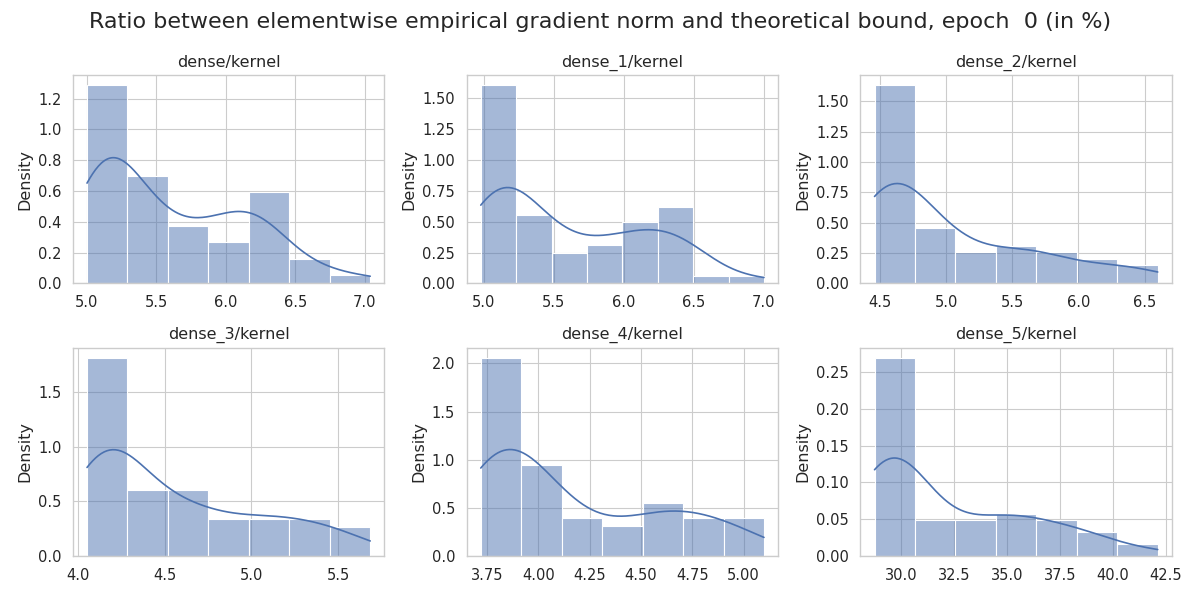
\includegraphics[width=\linewidth]{figures/histogram_ratios_epoch_0.png}
    \caption{\textbf{MLP Mixer on Cifar-10, first epoch.}}
    \label{fig:firstepochhist}
\end{figure}

\begin{figure}
    \centering
    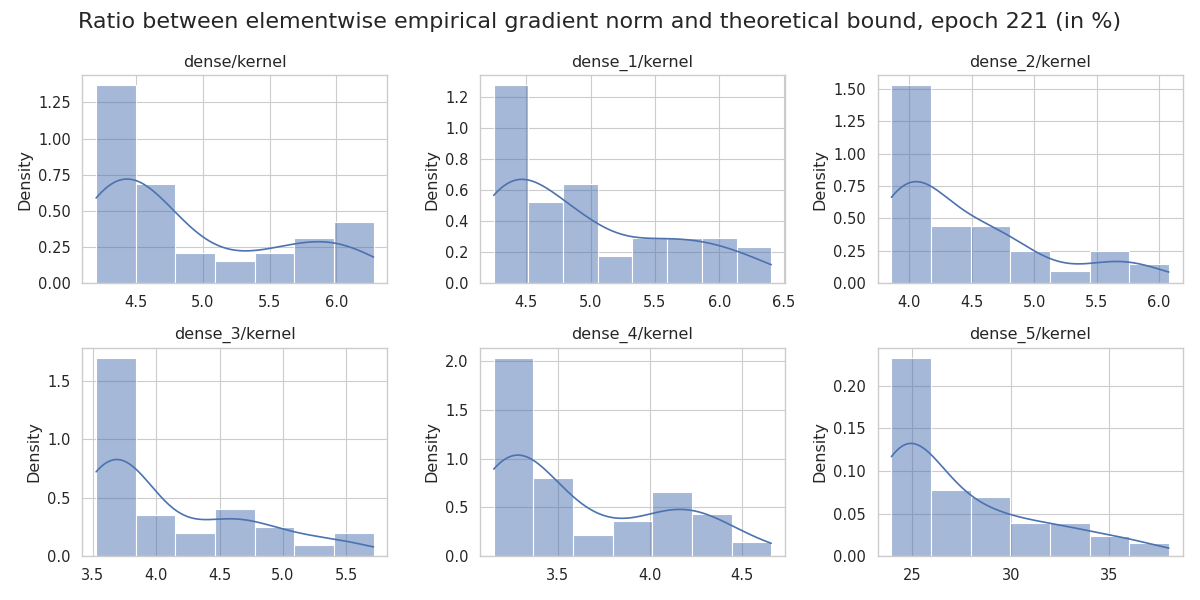
\includegraphics[width=\linewidth]{figures/histogram_ratios_epoch_221.png}
    \caption{\textbf{MLP Mixer on Cifar-10, last epoch.}}
    \label{fig:lastepochhist}
\end{figure}

We see that the last layer benefits from bounds that are quite tight (around 30\% to 50\%) whereas the tightness drops for the deeper  layers in MLP blocks (less than 10\%).  The explanation is that the bound 
\begin{equation} 
    \textcolor{paramcolor}{\left\|\Jac{f_d(\theta_d,x)}{\theta_d}\right\|_2}\leq K(f_d,\theta_d)\textcolor{forwardcolor}{X_{d-1}},
\end{equation}
might be overly pessimistic, because of the \textcolor{forwardcolor}{$X_{d-1}$} term, especially since Cauchy-Schwartz inequality is a ``best-case bound'' (i.e assuming that all vector involved in the inner product are co-linear), and do not account for the possible orthogonality between $x_d$ and the cotangent vector. Nonetheless, with a ratio of 4\% we see that the noise and the gradient norm are of similar amplitude as soon as the batch size exceed $1/0.04=25$ examples, which is clearly our case with batch sizes that easily exceed $2,500$ on Cifar-10.